\let\negthickspace\undefined
\documentclass[journal,12pt,twocolumn]{IEEEtran}
\usepackage{cite}
\usepackage{amsmath,amssymb,amsfonts,amsthm}
\usepackage{algorithmic}
\usepackage{graphicx}
\usepackage{textcomp}
\usepackage{xcolor}
\usepackage{txfonts}
\usepackage{listings}
\usepackage{enumitem}
\usepackage{mathtools}
\usepackage{gensymb}
\usepackage{comment}
\usepackage[breaklinks=true]{hyperref}
\usepackage{tkz-euclide} 
\usepackage{listings}
\usepackage{gvv}                                        
\def\inputGnumericTable{}                                 
\usepackage[latin1]{inputenc}                                
\usepackage{color}                                            
\usepackage{array}                                            
\usepackage{longtable}                                       
\usepackage{calc}                                             
\usepackage{multirow}                                         
\usepackage{hhline}                                           
\usepackage{ifthen}                                           
\usepackage{lscape}
\usepackage{tfrupee}

\newtheorem{theorem}{Theorem}[section]
\newtheorem{problem}{Problem}
\newtheorem{proposition}{Proposition}[section]
\newtheorem{lemma}{Lemma}[section]
\newtheorem{corollary}[theorem]{Corollary}
\newtheorem{example}{Example}[section]
\newtheorem{definition}[problem]{Definition}
\newcommand{\BEQA}{\begin{eqnarray}}
\newcommand{\EEQA}{\end{eqnarray}}
\newcommand{\define}{\stackrel{\triangle}{=}}
\theoremstyle{remark}
\newtheorem{rem}{Remark}
\begin{document}

\bibliographystyle{IEEEtran}
\vspace{3cm}

\title{10.5.3.15}
\author{EE23BTECH11062 - V MANAS}
\maketitle
\newpage

\bigskip

\renewcommand{\thefigure}{\theenumi}
\renewcommand{\thetable}{\theenumi}
\textbf{Question}:\\A contract on construction job specifies a penalty for delay of completion beyond a
certain date as follows: \rupee 200 for the first day, \rupee 250 for the second day, \rupee 300 for the third
day, etc., the penalty for each succeeding day being \rupee 50 more than for the preceding day.
How much money the contractor has to pay as penalty, if he has delayed the work by 30
days?\\
\textbf{Solution}:\\
Since the penalty is increasing \rupee 50 per day we can use the formula of an arithmetic progression.The formula for sum of first n numbers of an arithmetic progression is:
\begin{align}
    S_n=\frac{n}{2}[2a+(n-1)\times d]
\end{align}
\begin{figure}[h]
    \centering
    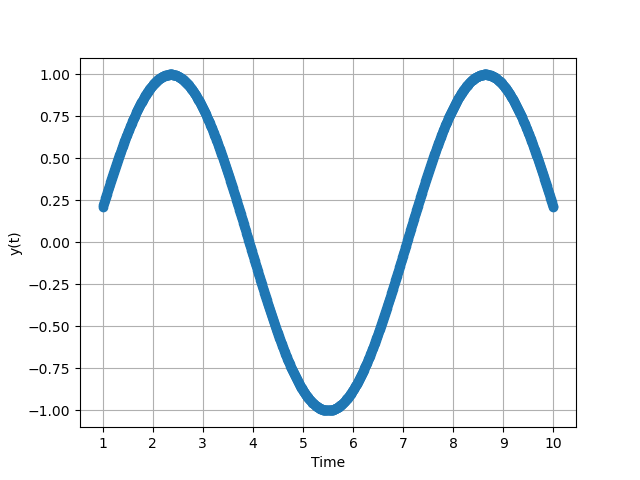
\includegraphics[width=1.1\linewidth]{/root/ee1205/assign10_5_3_15/figs/graph.png}
    \caption{Stem Plot of x(n)}
    \label{stemplot1}
\end{figure}
\begin{tabular}{|c|c|c|}
    \hline
    \textbf{Variable} & \textbf{Description} & \textbf{Value} \\
    \hline
    x(N) & General term($N_{th}$ term) & $x(0)+N\times d$\\
    \hline
    x(0) & First term of AP & 200\\
    \hline
    n & number of terms in the AP & 30\\
    \hline
    d & common difference in the AP & 50\\
    \hline
\end{tabular}
\begin{align}
S_n& =\frac{30}{2}[2\times 200+(30-1)\times 50]\\
S_n& =15[400+29\times 50]\\
S_n& =15[400+1450]\\
S_n& =15[1850]\\
S_n& =27750
\end{align}
$\therefore $The total amount of money that the contractor has to pay as penalty for the delay is \rupee 27750$
$
\end{document}
